\documentclass[border={10pt, 10pt, 10pt, 10pt}]{standalone}

\usepackage{tikz}
\usepackage{graphicx}
\usepackage{varwidth}

\renewcommand\familydefault{\sfdefault}

\begin{document}
\begin{tikzpicture}

\node at (0, 0) {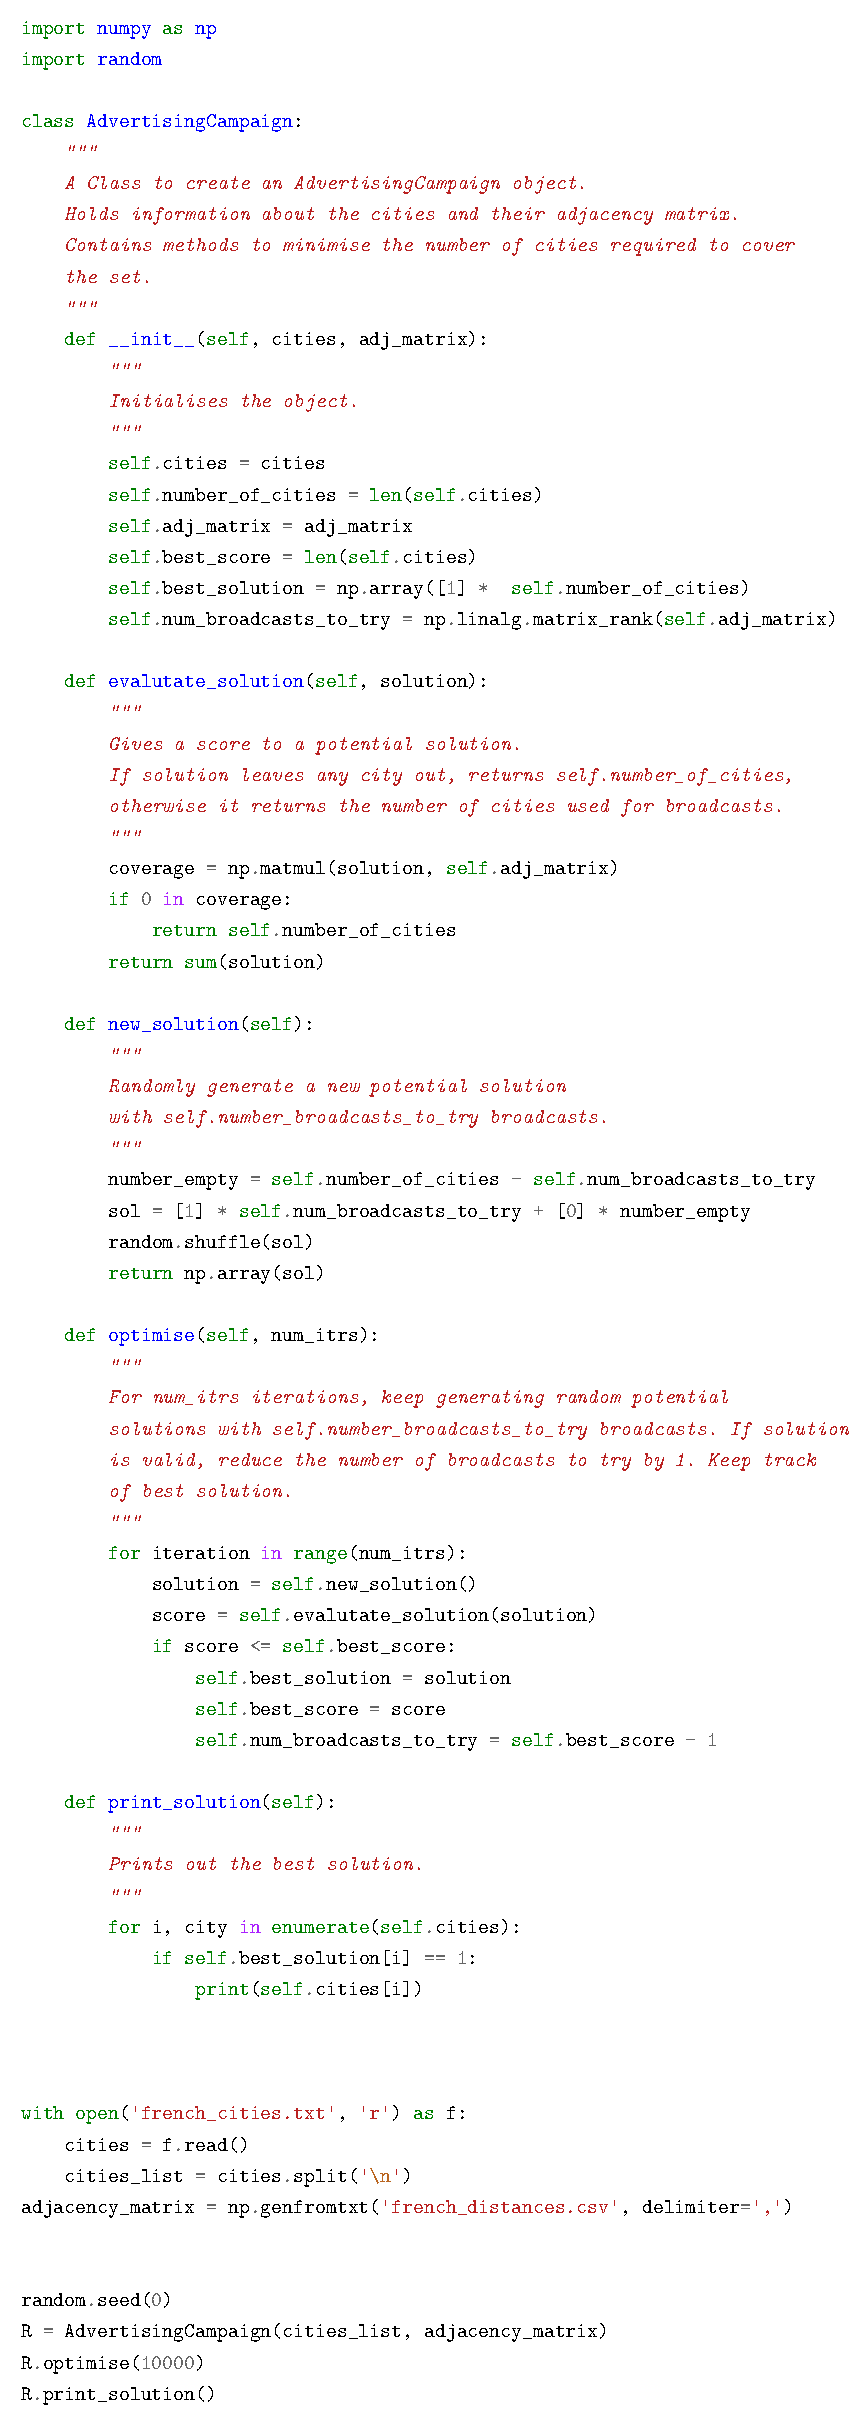
\includegraphics{concepts2.pdf}};

%%%%%%%%%%%%%
% LEFT SIDE %
%%%%%%%%%%%%%

% CLASSES
\draw[ultra thick, draw=red!50!black] (-7.75, 16.5) -- (-7.75, 18.75) -- (-5, 18.75);
\draw[ultra thick, dashed, draw=red!50!black] (-7.75, 16.5) -- (-7.75, 15);
\draw[ultra thick, dotted, draw=red!50!black] (-7.75, 15) -- (-7.75, 14);
\draw[ultra thick, draw=red!50!black] (-4.5, -18.7) -- (-7.25, -18.7) -- (-7.25, -19.15) -- (-4.5, -19.15);

% __INIT__
\draw[ultra thick, draw=green!50!black] (-5, 9.7) -- (-7.25, 9.7) -- (-7.25, 15.05) -- (-5, 15.05);

% METHODS
\draw[ultra thick, draw=blue!50!black] (-7.25, 8) -- (-7.25, 9.25) -- (-5, 9.25);
\draw[ultra thick, dashed, draw=blue!50!black] (-7.25, 8) -- (-7.25, 6.5);
\draw[ultra thick, dotted, draw=blue!50!black] (-7.25, 6.5) -- (-7.25, 5.5);

\draw[ultra thick, draw=blue!50!black] (-7.25, 2.3) -- (-7.25, 3.55) -- (-5, 3.55);
\draw[ultra thick, dashed, draw=blue!50!black] (-7.25, 2.3) -- (-7.25, 0.8);
\draw[ultra thick, dotted, draw=blue!50!black] (-7.25, 0.8) -- (-7.25, -0.2);

\draw[ultra thick, draw=blue!50!black] (-3, -6) -- (-5.75, -6) -- (-5.75, -6.55) -- (-3, -6.55);

\draw[ultra thick, draw=blue!50!black] (-4.5, -19.25) -- (-7.25, -19.25) -- (-7.25, -20.2) -- (-4.5, -20.2);

% SELF

\draw[ultra thick, draw=magenta!50!black] (-3.4, -6.6) -- (-3.4, -7) -- (-2.4, -7);
\draw[ultra thick, draw=magenta!50!black] (-4.3, -9.2) rectangle (-3.15, -7.6);



%%%%%%%%%%%%%%
% RIGHT SIDE %
%%%%%%%%%%%%%%

% ATTRIBUTES
\draw[ultra thick, draw=cyan!50!black] (-2.5, 9.7) -- (7.5, 9.7) -- (7.5, 13) -- (-2.5, 13);
\draw[ultra thick, draw=cyan!50!black] (-1.5, -7.6) -- (7.5, -7.6) -- (7.5, -9.2) -- (-1.5, -9.2);

% LIBRARIES
\draw[ultra thick, draw=orange!50!black] (-7, 19.2) -- (-2, 19.2) -- (-2, 20.5) -- (-7, 20.5);
\draw[ultra thick, draw=orange!50!black] (-3.5, 5.6) -- (3.5, 5.6) -- (3.5, 6.1);

% FILES
\draw[ultra thick, draw=yellow!50!black] (-2.5, -14.9) -- (7.5, -14.9) -- (7.5, -17.2) -- (-2.5, -17.2);


%% BOXES
\draw[ultra thick, draw=red!50!black, fill=red!10!white] (-24, 21.5) rectangle (-14, 11.5);
\draw[ultra thick, draw=green!50!black, fill=green!10!white] (-24, 10.5) rectangle (-14, 0.5);
\draw[ultra thick, draw=blue!50!black, fill=blue!10!white] (-24, -0.5) rectangle (-14, -10.5);
\draw[ultra thick, draw=magenta!50!black, fill=magenta!10!white] (-24, -11.5) rectangle (-14, -21.5);

\draw[ultra thick,  draw=cyan!50!black, fill=cyan!10!white] (24, 21.5) rectangle (14, 11.5);
\draw[ultra thick, draw=orange!50!black, fill=orange!10!white] (24, 10.5) rectangle (14, 0.5);
\draw[ultra thick, draw=yellow!50!black, fill=yellow!10!white] (24, -0.5) rectangle (14, -10.5);
\draw[ultra thick, fill=black!10!white] (24, -11.5) rectangle (14, -21.5);

%% STEMS
\draw[ultra thick, draw=red!50!black] (-7.75, 17.75) -- (-8.6, 17.75) -- (-8.6, 16.5) -- (-14, 16.5); % classes
\draw[ultra thick, draw=red!50!black] (-7.25, -18.9) -- (-8.6, -18.9) -- (-8.6, 16.5); % classes
\draw[ultra thick, draw=blue!50!black] (-7.25, 8.6) -- (-11.3, 8.6) -- (-11.3, -5.5) -- (-14, -5.5); % methods
\draw[ultra thick, draw=blue!50!black] (-7.25, 2.9) -- (-11.3, 2.9); % methods
\draw[ultra thick, draw=blue!50!black] (-7.25, -19.7) -- (-11.3, -19.7) -- (-11.3, -5.5); % methods
\draw[ultra thick, draw=blue!50!black] (-5.75, -6.275) -- (-11.3, -6.275); % methods
\draw[ultra thick, draw=green!50!black] (-7.25, 12.4) -- (-12.65, 12.4) -- (-12.65, 5.5) -- (-14, 5.5); % init
\draw[ultra thick, draw=magenta!50!black] (-3.4, -7) -- (-9.95, -7) -- (-9.95, -16.5) -- (-14, -16.5); % self
\draw[ultra thick, draw=magenta!50!black] (-4.3, -8.4) -- (-9.95, -8.4); % self
\draw[ultra thick, draw=cyan!50!black] (7.5, -8.4) -- (9.95, -8.4) -- (9.95, 16.5) -- (14, 16.5); % attributes
\draw[ultra thick, draw=cyan!50!black] (7.5, 11.35) -- (9.95, 11.35); % attributes
\draw[ultra thick, draw=orange!50!black] (-2, 19.85) -- (8.6, 19.85) -- (8.6, 5.5) -- (14, 5.5); % libraries
\draw[ultra thick, draw=orange!50!black] (3.5, 5.85) -- (8.6, 5.85); % libraries
\draw[ultra thick, draw=yellow!50!black] (7.5, -16.05) -- (11.3, -16.05) -- (11.3, -5.5) -- (14, -5.5); % for


%% TITLES/TEXT
\node[text=red!50!black] at (-19, 20.5) {\huge CLASSES};
\node at (-19.5, 17.5) {\Large{\begin{varwidth}{9cm}
    \begin{itemize}
      \item A recipe for creating objects,
      \item A structure to hold information,
      \item Many objects can be created from same recipe,
      \item Consists of methods and attributes.
    \end{itemize}\end{varwidth}
}};

\node[text=green!50!black] at (-19, 9.5) {\huge \texttt{\_\_init\_\_}};
\node at (-19.5, 7) {\Large{\begin{varwidth}{9cm}
    \begin{itemize}
      \item A methods that is called when the object is created,
      \item Its arguments are used to create the object,
      \item Usually sets a number of attributes.
    \end{itemize}\end{varwidth}
}};

\node[text=blue!50!black] at (-19, -1.5) {\huge METHODS};
\node at (-19.5, -5.2) {\Large{\begin{varwidth}{9cm}
    \begin{itemize}
      \item Functions that are associated with an object,
      \item Called with `\texttt{.}',
      \item Can call other methods and attributes,
      \item First argument must be \texttt{self},
      \item Can return something or change the object.
    \end{itemize}\end{varwidth}
}};

\node[text=magenta!50!black] at (-19, -12.5) {\huge \texttt{self}};
\node at (-19.5, -14) {\Large{\begin{varwidth}{9cm}
    \begin{itemize}
      \item A way of accessing information associated with the object.
    \end{itemize}\end{varwidth}
}};

\node[text=cyan!50!black] at (19, 20.5) {\huge ATTRIBUTES};
\node at (19, 17) {\Large{\begin{varwidth}{9cm}
    \begin{itemize}
      \item Variables that are associated with the object,
      \item Accessed with `\texttt{.}',
      \item Can be changes or created by methods,
      \item Set or changed with \texttt{self}.
    \end{itemize}\end{varwidth}
}};

\node[text=orange!50!black] at (19, 9.5) {\huge LIBRARIES};
\node at (19, 7) {\Large{\begin{varwidth}{9cm}
    \begin{itemize}
      \item Packaged, pre-written code,
      \item Must be imported with \texttt{import},
      \item A wide variety available.
    \end{itemize}\end{varwidth}
}};

\node[text=yellow!50!black] at (19, -1.5) {\huge FILES};
\node at (19, -3.5) {\Large{\begin{varwidth}{9cm}
    \begin{itemize}
      \item Can load external data,
      \item Many different ways of reading these.
    \end{itemize}\end{varwidth}
}};

\node[text=black!50!black] at (19, -12.5) {\huge OTHER?};
\node at (16, -15) {\LARGE \texttt{with}};
\node at (21, -16) {\LARGE \texttt{enumerate}};
\node at (16, -17) {\LARGE Seeds};

\end{tikzpicture}
\end{document}